\documentclass[11pt,journal,compsoc]{IEEEtran} % Set to 11pt if we ever have the luxury of doing so.
%\usepackage[T1]{fontenc}
\usepackage{graphicx}
\usepackage[cmex10]{amsmath}
\usepackage{fixltx2e}
\graphicspath{ {img/} }

% IMPORTANT:
%  This document class uses logical paragraphs rather than manual ones.
%  In other words, use a blank line instead of \\ to start a new paragraph.

\begin{document}
\title{Programatically Predicting [Bus] Occupancy\\
{\large Undergraduate Independent Research Report}}
\author{Daniel~Bordak, Erin~Corrado, Revan~Sopher, and Ashley~Weaver}

\IEEEtitleabstractindextext{% Comment to prevent unwanted space
\begin{abstract}
In this study we address the problem of programatically predicting bus occupancy.
We approach this in two ways: by using publicly available GPS positions to calculate stop time, and by using promiscuous Wi-Fi to count devices.
While the stop time approach proved unfruitful due to the significant time requirement in establishing a benchmark by which to interpret the data, the Wi-Fi approach yielded an accurate model once we compensated for noise.
We conclude by suggesting modifications to the experiment, and the application of this methodology to the determination of occupancy of other locales.
\end{abstract}}

\maketitle

\section{Motivation}

\IEEEPARstart{D}{ue to}
the periodic nature of class schedules, students at Rutgers tend to move between campuses during certain known time intervals during the day.
This leads to predictable migratory patterns.
However, the bus schedule does a poor job of taking student schedules into account -- for example, on Livingston campus, buses on the route to College Avenue can often be found lined up at the stops consecutively, while the buses on the route to Busch are much rarer.
To make matters worse, the Busch buses are usually packed to capacity between class periods.
The aim of this project is to develop a system for better predicting the demand for buses, such that an empirical argument for the optimization of the bus schedule might be made.

\section{Approach}

In order to facilitate simultaneous contributions from all four team members, we approached the problem in two manners: by directly collecting data about number of riders vs. stop time, and by measuring number of devices on the bus.
Two students were assigned to work on each approach.
Ultimately, we planned to combine results into a single prediction method.

\subsection*{Stop Length Inference}

	In this approach, we planned to establish a correlation between the length of time a bus spends at a stop and the number of passengers currently aboard.
Our initial theory was that a bus nearing capacity would take longer at stops due to the larger number of riders entering and exiting.
	Every Rutgers bus periodically reports its position, velocity, and destination to an online service -- nextbus.com's Public API.
	This service is free to use, its information is publicly available. %TODO: Add example XML
    As such, using it would not require any hardware or observers on the bus, allowing for cheap, large-scale execution.
	We first tried to measure the strength of this correlation; if we could prove a strong positive correlation, we could use the bus travel data to measure length of stops, and therefore predict occupancy.
	By running the analysis on a log of travel data, we could predict occupancy across a significantly larger domain and for theoretically no cost.

	In order to establish a correlation between stop length and bus occupancy, we followed a bus on its circuit, recording data about its stops. Specifically, we recorded the number of people boarding or departing the bus, the length of the stop, and what time it was.

\subsection*{Promiscuous WiFi}

	In this approach, we used the inherent correlation between the number of smartphones on the bus and the number of passengers; it is reasonable to assume that more devices means more passengers, since the devices travel with the passengers.
	We hold that this correlation is fundamental enough to not require investigation, unlike the other approach.

    Data collection was performed with a laptop running Linux, equipped with a typical 802.11n wireless card and a GPS sensor.
	The computer ran the wireless card in monitor mode.
	In normal operation, a wireless card will receive every packet in the vicinity, but discard those that are not specifically addressed to it; in monitor mode all received packets are transmitted to the operating system regardless of intended recipient. With this setup, we ran the following command:
	\begin{verbatim}
		tcpdump -e
	\end{verbatim}
	This command logs the headers of every packet that the wireless card sees, thus uniquely identifying every active device in the area.
	The strength of signals is also recorded, so we can choose to ignore packets below a certain decibel strength.
	We rode a bus along its route, logging packets and stop times. %TODO: Add example bits of a log file, with the addresses replaced with ``XX:XX:XX:XX:XX''

\section{Graph Production}

\subsection*{Preprocessing}

	The raw output from running tcpdump contains many irrelevant details -- fields like the type of packet, or the antenna used.
	As such, our first step in graph production was to preprocess this data, preserving only the information relevant to our goal.
    The main data of interest was the list of MAC addresses seen in a given packet.
    Each of these addresses can take one of four roles: Source, Destination, Transmitter, and Receiver.
    Every packet will have some, but not all, of these types of addresses.
    Since each line of tcpdump raw output represents a packet, our log files are first parsed line by line, each line individually stored as a Python Dict -- otherwise known as a Hash Map.
    These Dicts hold the four potential addresses, the packet's strength, and what time it was sent at (in microseconds).
    All the other information was disregarded; ignoring information during preprocessing is the simplest way of removing it from the data.

A few special considerations needed to be made during this step:
    \begin{itemize}
    \item Packets may not have a strength field.
      To make data handling easier later on, these are assigned a strength of zero.
      This is easier since it can be filtered out later simply by checking that the strength field is nonzero; a zero strength appearing naturally is impossible. 
    \item Some lines contain only the address of a router, with no particular destination in mind.
      These are broadcast packets, sent to notify devices of the router's existence.
      Since we are monitoring personal devices, not routers, these lines are ignored, and the address identified as a router is flagged for future filtering.
    \item Since MAC addresses are usually unique device identifiers, they could potentially be used to identify device owners.
      This kind of risk could subject our study to human subject regulations.
      In order to avoid this risk, addresses are saved into the Dicts as index numbers (starting from zero) rather than the actual address.
      This way, we can still differentiate between multiple devices without having to worry about our data being used for morally questionable purposes.
    \end{itemize}
    At the end of the parsing process, the Dicts are dumped into a JSON output file.
    JSON is a open standard data interchange format.
    Using JSON made utilizing the data much easier when it came to producing the graphs; most languages, Python included, have a standard library implementation for JSON, eliminating the effort spent in re-parsing the data. % TODO: Add example JSON output -- re-run raw2json with prettyprint on.

\subsection*{Filtering}
    The preprocessing done above is only performed once per dataset.
    Therefore, any sort of filtering that might change between two graphs must be done immediately before the construction of the graph.
    We built four filters to be run at this stage:
    \begin{itemize}
    \item The Strength filter removes packets below a given strength threshold.
      For example, a strength filter of -50 would filter out packets of -51dB.
    \item The Zero-Strength filter removes packets which have a strength field of zero.
      These packets correspond to tcpdump output lines missing a strength field, as mentioned above in the preprocessing section.
    \item The Router filter removes any addresses which were flagged as routers during the parsing step.
      It also removes any packets which would no longer contain any addresses after the previous is performed.
    \item The End Time filter removes any packets past a certain time.
      This is desirable when you only want to look at a part of a dataset.
      We never produced a corresponding Start Time filter since the need never arose.
    \end{itemize}

\subsection*{Graphing}
    For the construction of the graphs, a few additional libraries were needed: Numpy, Pandas, and Matplotlib.
    Numpy is an advanced mathematical library for Python, and Pandas is a library built on top of Numpy to provide high-performance data structures.
    We used these for data analysis.
    Matplotlib is a 2D plotting library, which we used to generate the graphs. 
    In order to simplify the graph production process, we made individual scripts for each graph type, plus a meta-script to make a united interface.
    This meta-script reads a JSON file obtained from the preprocessing step, imports the data into a Pandas DataFrame (which can be thought of as a complicated 2D array), and sends this off to be filtered, as explained in the filtering step.
    After the data has been filtered, it is handed off to one of the six plotting scripts:
    \begin{itemize}
    \item The Packet and Unique plots were created by generating an array of 3-second bins and adding the appropriate statistic to the bins.
      In the case of the packet plot, this was simply the number of packets found over those three seconds; the bin is simply an integer.
      In the case of the unique plot, however, the bin is a mathematical set holding the MAC addresses seen over the three second period.
      After the entirety of the three seconds are parsed, the bin is assigned the length of the set.
    \item The First-Last Grid, Packet Histogram, and Vector plot were all created by checking the data set for each address.
      The first time each MAC address is encountered, it is added to a list with an initial value of the time it was seen as both its first and last time seen, and seen-count of one.
      Each additional time an address is seen, its last time seen value is updated to the current time, and its seen-count is incremented.
      In the Grid, the addresses are graphed using the first time seen as the x-value and the last time seen as the y-value.
      In the packet histogram, packets which fulfill the requirement of \(t_{first} + t_{max} - t_{last} < 120\) are selected, where \(t_{max}\) is the total observation time.
      These selected packets are then graphed with their y-values set as their seen-count.
      To make the graph easier to interpret, the y-axis was made to be logarithmic, and the addresses are sorted by their y-values.
      For the Vector plot, first an array of zeros was initialized with length equal to the length of observation in seconds.
      For each packet, every value between \(t_{first}\) and \(t_{last}\) was incremented.
      The resulting array was plotted as a step function, with the x-axis being its indices.
    \item The segment plot is the most complicated plot we generated.
      First, a list of mathematical sets are generated, one for each stop.
      These sets are called the stop-sets.
      The stop-sets are populated with the MAC addresses seen during the corresponding stop.
      Next, a second list of mathematical sets are generated, again, one for each stop.
      These sets are called the intersect-sets.
      The intersect-sets are filled with the intersect between the stop-set of the same index value, and every other stop-set, combined by union.
      For instance, intersect-set 2 would contain
      \begin{multline*}
      \left(stop_2 \cap stop_0\right) \cup \left(stop_2 \cap stop_1\right) \cup \\
      \left(stop_2 \cap stop_3\right) \cup \dots \cup \left(stop_2 \cap stop_n\right)
      \end{multline*}
      The length of each intersect-set is considered to be the number of people on the bus at the stop.
      A special exception is made for the intersect of stop-set 0 and stop-set n.
      This set represents addresses present both at the beginning of the ride and the end.
      No normal student would do this -- this would consist only of ourselves and possibly devices present around this stop.
      As such, this set is instead subtracted from all other intersect sets; it is likely garbage.
      Afterward, we add a flat value of 2 to every stop, representing the two of us we filtered out.
    \end{itemize}
    Some graphs also had the actual number of people on the bus, as observed, overlaid.
    This overlay was generated with a simple step function, using the value at n+1 as the value for the line between n and n+1.

\pagebreak

\section{Results}

\subsection*{Stop Length Inference}
	\begin{figure}[!t]
      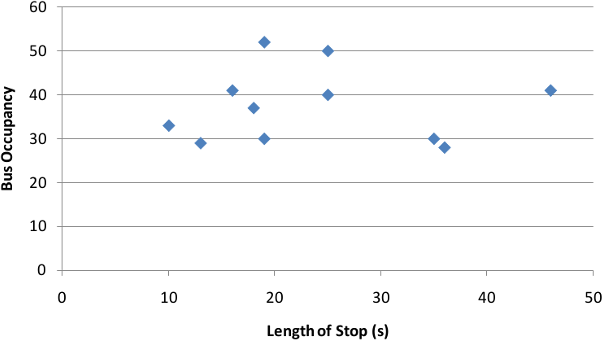
\includegraphics[width=0.5\textwidth]{occupancy}
      \caption{Bus Occupancy as a function of Stop Length} %TODO: Clarify whether this is for the following or preceeding stop. I don't actually remember.
      \label{fig:occ}
	\end{figure}
                         
    \begin{figure}[!t]
	  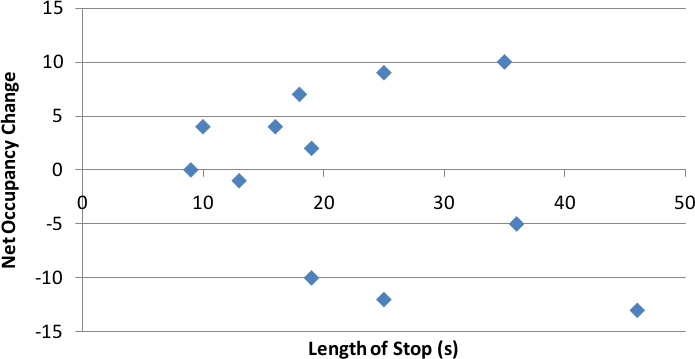
\includegraphics[width=0.5\textwidth]{netdelta}
      \caption{Net Delta Occupancy as a function of Stop Length}
      \label{fig:netdelta}
	\end{figure}

    Analyzing this data (fig.~\ref{fig:occ}), it quickly became apparant that stop length does not have any correlation to occupancy.
	This makes sense, because the number of sedentary riders does not cause slowdowns; rather, the relevant metric is the number of people entering or exiting the bus.
	Plotting the net occupancy change as a function of stop length (fig.~\ref{fig:netdelta}) was also inconclusive, as the longer stops could signify either positive or negative changes.
	From stop timings alone, we would not be able to predict the direction of change.

    \pagebreak
    
	\begin{figure}[!t]
	  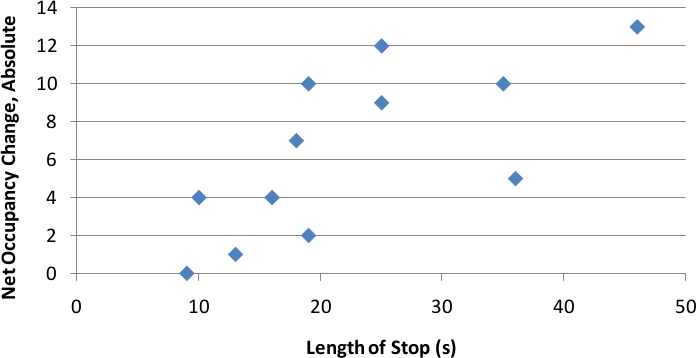
\includegraphics[width=0.5\textwidth]{absdelta}
      \caption{Absolute Delta Occupancy as a function of Stop Length}
      \label{fig:absdelta}
	\end{figure}

    \begin{figure}[!t]
	  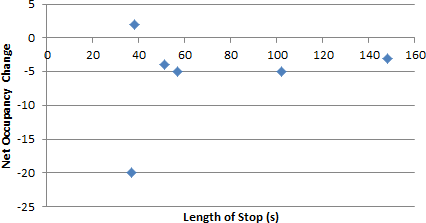
\includegraphics[width=0.5\textwidth]{onestopcrop}
      \caption{Net Delta Occupancy, Single Stop}
      \label{fig:onestop}
	\end{figure}
    
	Absolute change (fig.~\ref{fig:absdelta}), however, shows a much stronger correlation than either of the previous graphs.
    Net change is not a useful metric on its own, but if it could be proven that certain bus stops tended to have a generally positive or negative net change, we could predict the sign of the change and thus the occupancy changes over time.
	In other words, if more people tend to get on at a given stop than get off, a longer stop here means a large positive change to the number of passengers.
	Conversely, a stop which is associated mostly with disembarking, a long stop would mean a large negative change.

	To test this, we waited at a single bus stop and counted the number of passengers entering and leaving each bus on a certain route, and the length of the stops (fig.~\ref{fig:onestop}).
	Data for this experiment was slower to collect, as the buses were spaced out.
	This data suggests that this particular bus stop is predominantly a destination, rather than a starting point; longer stops here, then, would imply a net decrease in number of riders.
    
	However, the data collected is insufficient to draw these conclusions; there can be significant variation depending on time and day of the week.
	This data collection would need to be repeated at every bus stop, on a variety of days and times, in order to provide the required basis of prediction.
	This clearly increases the time requirement to well beyond the scope of this study.
	
	Thus, while the preliminary foray suggests that this approach is tentatively successful, it is not feasible for this study.
	We move on to our next approach.

\subsection*{Promiscuous WiFi}
    
	\subsubsection*{Packet Plot}
		\begin{figure*}[!t]
		  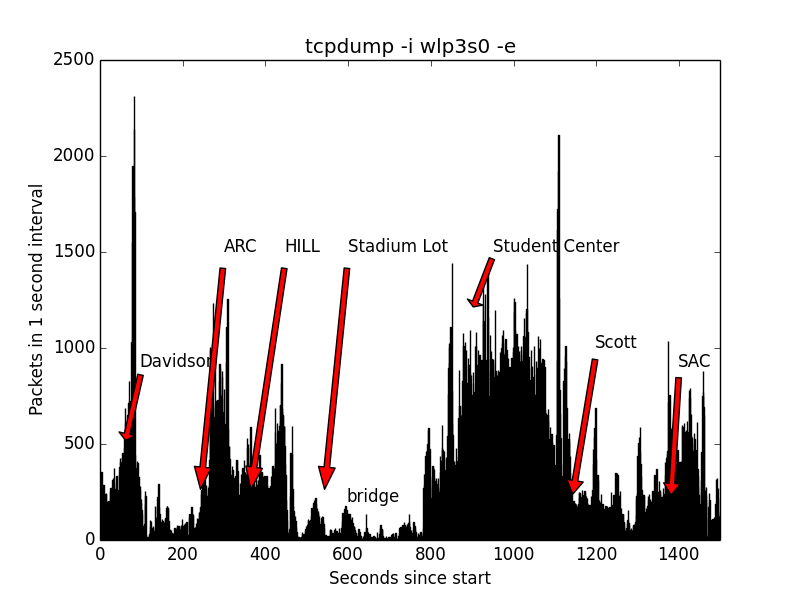
\includegraphics[width=\textwidth]{packets}
          \caption{Packets detected per 3-second bin}
          \label{fig:buspackets}
		\end{figure*}

		Plotting the number of packets in a histogram with three second bins (fig.~\ref{fig:buspackets}), we see that there are visible differences between stops.
		This roughly lines up to the expected traffic around each stop -- stops like the BCC, Hill, the ARC, and the entirety of College Avenue have a large amount of traffic, while stops near the Visitor's Center and Werblin have very little.

	\subsubsection*{Unique MAC Plot}

		Network traffic is not a good indicator of occupancy, however, because it represents the amount of activity, rather than the number of actors; a single person transmitting a large amount of data may be interpreted as multiple people with the Packet Plot.
		As such, our next step was to switch out ``number of packets'' for ``number of unique MAC addresses''.
		The Router filter would be used here, since we don't want to count routers among the number of riders.

		\begin{figure*}[!t]
		  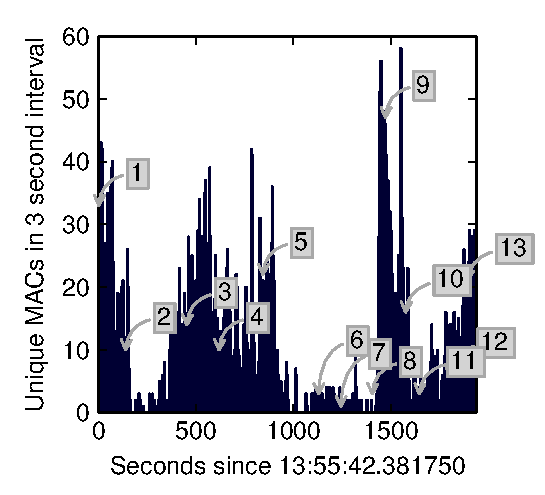
\includegraphics[width=\textwidth]{unique}
          \caption{Unique MAC addresses detected per 3-second bin}
          \label{fig:busunique}
		\end{figure*}

		The values on this plot differ noticeably between stops.
		However, this is not due to occupancy; there are clearly not nearly that many people on the bus.
		Instead, it seems that the shape of the plot is primarily influenced by the proximity to routers -- the portions of the bus loop by athletic fields and between campuses has nearly no data.

	\subsubsection*{First-Last Grid Plot}
		In order to establish which devices were on the bus, we plotted the time of the first and last occurrence of each device:

		\begin{figure*}[!t]
		\includegraphics[width=\textwidth]{bus-grid-fixed}
		\end{figure*}

		Each point here represents a unique device, where the x-coordinate is the time of the first sighting, and the y-coordinate is the time of the last sighting.
		Thus, the high concentration of data points along the line \(y=x\) represents the transient devices, most likely people the bus was passing by.
		The clump of data points in the top left corner of the plot represents devices which were seen throughout the journey.
		These are most likely our own devices, or stationary devices around the geographically identical first and last stops.

	\subsubsection*{Presence Vector Plot}
		In an attempt to minimize noise from the above transient devices and to compensate for the lack of traffic in uninhabited areas, we construct a plot similar to the previous. % This isn't a complete thought
		For every address we encountered in the collection, we create a vector defined by the following function:
		\begin{equation*}
		f(t) = \begin{cases}
			1 & t_{firstSeen} \le t \le t_{lastSeen}\\
			0 & otherwise
		\end{cases}
		\end{equation*}

		We sum these vectors into a single vector, where the value at any point indicates how many devices we can infer are presently on the bus.

		\begin{figure*}[!t]
		\includegraphics[width=\textwidth]{bus-vectors-wide}
		\end{figure*}

		Overlaid on this plot is the step function corresponding to the observed number of riders.
		It is scaled differently, as there is approximately a three time difference between the devices seen and the people riding.
		
		We see that there appears to be an excellent correlation here, with the exception of the 400-700 second segment. % uhh... what about 0-400? That's also pretty bad.
		This segment corresponds to the entrance to the College Avenue campus, a highly concentrated area which appears to have contributed considerable noise.
		We do see, however, that the two changes in occupancy in this region seem to correspond to peaks in the traffic -- this means that the traffic is probably a flat-rate higher in that area, which we can account for in prediction.
		
		Thus, we can conclude that this approach is successful. % I don't know about that, it seems really shaky to just declare that here.

%\section{Conclusion}
%	From the data above, we determined that the occupancy of a bus could be predicted by observing data traffic with some sensor placed on the bus.
%	We can filter out some of the irrelevant data by ignoring any signals below a certain strength.
%	This is the most feasible method, but requires external assistance with installation of devices.

\section{Future Work}
    
\subsection*{Continuation of Benchmark}
	The Stop Length Inference approach seemed promising, but we would need to benchmark every stop several times in order to be able to know which direction of occupancy change a long stop indicates.
    As such, there is substantial opportunity to complete this benchmarking in order to complete that approach.

\subsection*{Alternative Approach}
	The largest problem with the interception of packets is outside noise.
	To address this, we would like to install an access point on the bus, with the same SSID as the campus Wi-Fi so that smart phones would automatically connect.
	We could then listen only to communications with this access point, eliminating outside traffic.
	
Optimally, the routers would be officially installed and serve mobile data.
	This is naturally expensive and thus unlikely.
	Any unofficial access points installed would be an explicit violation of the terms of use of the Rutgers networks, and thus unfeasible as well.

We could also replace the laptop in our setup with a smaller unit to be installed in the buses, to collect data for longer periods of time.
	Running several of these units would allow us to collect enough data to make occupancy predictions.

\subsection*{Alternative Application}
	While we initially set out to programatically predict the occupancy of buses, the Promiscuous Wi-Fi approach is also applicable to the determination of the occupancy of other scenarios.
	To demonstrate, we ran tcpdump for twenty minutes during a lecture, and followed a similar analysis procedure.
	The concept of "stops" doesn't apply to this situation; however, we can still derive interesting results.

	\begin{figure*}[!t]
	  \includegraphics[width=\textwidth]{lecture-grid}
      \label{fig:probgrid}
	\end{figure*}

	As before, the points around \(y=x\) consist of transient devices.
	The points in the clump to the top right is probably due to a buildup of students outside the lecture hall awaiting the following class.
	The points in the clump to the top left represent the devices that were present for the duration of the capture.
	
	There were exactly 106 students in the lecture hall during this collection; while determining the exact boundaries is of a complexity outside the scope of this project, the clump in the top left contains approximately 100 points.
	This suggests that this approach does generate an accurate count of the lecture hall occupancy.

	\begin{figure*}[!t]
	  \includegraphics[width=\textwidth]{packethist-sorted}
      \label{fig:probhist}
	\end{figure*}

	In this plot we see that we can partition devices into classes based on how frequent the packets.
	While a small number of devices were generating enormous amounts of network traffic with millions of packets, others generated orders of magnitude fewer.
	
	This suggests another interesting path of inquiry: monitoring the interest of an audience based on network traffic.
	The assumption here is that a bored audience is more likely to cause network traffic by web browsing.

\pagebreak

\appendix[Team Member Contributions]
Daniel Bordak
\begin{itemize}
  \item Collected tcpdump and classroom data
  \item Created tcpdump output parser used in all plots (not yet in report)
  \item Optimized graph plotting functions for speed and maintainability
  \item Cowrote First-Last Grid Plot
  \item Cowrote Segments Plot (not in report)
  \item Rewrote Unique Device Plot and Packet Plot to allow for different binsizes (not yet in report)
  \item Wrote script to generate stop annotations, used on most plots.
  \item Wrote sections of the report pertaining to the creation of plots
\end{itemize}
Erin Corrado
\begin{itemize}
  \item Collected bus and classroom data
  \item Cowrote First-Last Grid Plot
  \item Wrote length/occupancy correlation plot
  \item Cowrote poster
  \item Cowrote Packet Histogram
\end{itemize}
Revan Sopher
\begin{itemize}
  \item Wrote Proposal
  \item Collected tcpdump data
  \item Wrote Raw Packet Plot
  \item Wrote Unique Device Plot
  \item Cowrote Segments Plot (not in report)
  \item Wrote Vector Plot
  \item Wrote Report
\end{itemize}
Ashley Weaver
\begin{itemize}
  \item Collected bus data
  \item Cowrote Poster
  \item Commented on report
\end{itemize}
\end{document}
